% ============================================================
%  main.tex  —  Asosiy fayl (standalone Overleaf loyiha)
%  Modellashtirish darsligi, I Bob
%  Muallif: Matematik, Professor
% ============================================================
\documentclass[12pt, a4paper]{report}

% --- Preamble fayllarini yuklash ---
% ============================================================
%  packages.tex  —  Barcha paketlar shu yerda e'lon qilinadi
% ============================================================

% --- Kodlash va shrift ---
\usepackage[T1]{fontenc}
\usepackage[utf8]{inputenc}
\usepackage{lmodern}
\usepackage{microtype}

% --- Sahifa o'lchamlari ---
\usepackage[a4paper, top=2.5cm, bottom=2.5cm, left=3cm, right=2.5cm]{geometry}

% --- Matematika ---
\usepackage{amsmath}
\usepackage{amssymb}
\usepackage{amsthm}
\usepackage{mathtools}
\usepackage{bm}

% --- Teorema muhitlari ---
\usepackage{thmtools}

% --- Grafiklar ---
\usepackage{tikz}
\usepackage{pgfplots}
\pgfplotsset{compat=1.18}
\usetikzlibrary{
  arrows.meta,
  angles,
  quotes,
  calc,
  patterns,
  patterns.meta,
  decorations.pathmorphing,
  decorations.markings,
  decorations.pathreplacing,
  intersections,
  backgrounds,
  fit,
  shapes.geometric,
  math
}
\usepackage{subcaption}

% --- Jadvallar ---
\usepackage{booktabs}
\usepackage{array}
\usepackage{tabularx}

% --- Ranglar ---
\usepackage{xcolor}

% --- Qutichalar ---
\usepackage[most]{tcolorbox}
\tcbuselibrary{theorems, skins, breakable}

% --- Ro'yxatlar ---
\usepackage{enumitem}

% --- Havolalar ---
\usepackage[
  colorlinks = true,
  linkcolor  = blue!55!black,
  citecolor  = green!45!black,
  urlcolor   = blue!65!black
]{hyperref}

% --- Adabiyotlar ---
\usepackage[backend=biber, style=alphabetic, sorting=nyt, maxbibnames=99]{biblatex}
\addbibresource{bib/references.bib}

% --- Boshqalar ---
\usepackage{setspace}
\usepackage{caption}
\captionsetup{font=small, labelfont=bf}

% ============================================================
%  macros.tex  —  Maxsus buyruqlar, TikZ uslublari, ranglar
% ============================================================

% ---  Sonlar to'plamlari ---
\newcommand{\R}{\mathbb{R}}
\newcommand{\N}{\mathbb{N}}
\newcommand{\Q}{\mathbb{Q}}
\newcommand{\Z}{\mathbb{Z}}
\newcommand{\Qplus}{\mathbb{Q}_{+}}
\newcommand{\Rplus}{\mathbb{R}_{+}}

% --- Yuza belgisi ---
\newcommand{\Sarea}{S}
\newcommand{\Area}[1]{S\!\left(#1\right)}

% --- Qisqacha matematik buyruqlar ---
\newcommand{\half}{\tfrac{1}{2}}
\newcommand{\limn}{\lim_{n\to\infty}}
\newcommand{\eps}{\varepsilon}
\newcommand{\To}{\longrightarrow}
\newcommand{\abs}[1]{\left|#1\right|}

% ---- Ranglar (akademik palet: kulrang + ko'k aksent) ----
\definecolor{fillA}{RGB}{173, 216, 230}    % och ko'k
\definecolor{fillB}{RGB}{220, 220, 220}    % kulrang
\definecolor{fillC}{RGB}{198, 230, 190}    % och yashil
\definecolor{fillD}{RGB}{255, 230, 180}    % och sariq
\definecolor{geomblue}{RGB}{0,  90, 150}   % to'q ko'k chiziq
\definecolor{geomgray}{RGB}{70, 70,  70}   % to'q kulrang chiziq
\definecolor{accred}{RGB}{160, 20,  20}    % qizil aksent
\definecolor{dimclr}{RGB}{100,100,100}     % o'lcham chiziqlari
\definecolor{boxbg}{RGB}{240, 245, 255}    % formula qutisi foni

% ---- TikZ global uslublari ----
\tikzset{
  % Asosiy geometrik chiziq
  geomline/.style    = {thick,  draw=geomblue},
  geomdash/.style    = {dashed, draw=geomblue!70, thick},
  thickgeom/.style   = {very thick, draw=geomblue},
  % To'ldirilgan shakllar
  shapeA/.style  = {fill=fillA, draw=geomblue, thick},
  shapeB/.style  = {fill=fillB, draw=geomgray, thick},
  shapeC/.style  = {fill=fillC, draw=geomgray!80, thick},
  shapeD/.style  = {fill=fillD, draw=geomgray!80, thick},
  % O'q chiziqlari
  axisline/.style    = {-Stealth, thin, black!60},
  % O'lcham chiziqlari (dimension lines)
  dimline/.style     = {Stealth-Stealth, thin, dimclr},
  dimlinelabel/.style= {font=\small, dimclr},
  % Nuqtalar
  dotpt/.style       = {circle, fill=geomblue, inner sep=1.5pt},
  dotred/.style      = {circle, fill=accred,   inner sep=1.5pt},
  % Etiketlar
  lab/.style         = {font=\small, inner sep=1pt},
  labmath/.style     = {font=\small},
}

% ---- tcolorbox uslublari ----
\tcbset{
  formulabox/.style = {
    enhanced,
    colback  = boxbg,
    colframe = geomblue,
    fonttitle= \bfseries\small,
    boxrule  = 0.8pt,
    arc      = 3pt,
    breakable
  },
  resultbox/.style = {
    enhanced,
    colback  = fillA!40,
    colframe = geomblue!70,
    fonttitle= \bfseries\small,
    boxrule  = 0.7pt,
    arc      = 3pt
  },
}

% ============================================================
%  theorems.tex  —  Barcha teorema muhitlari
% ============================================================

% amsthm allaqachon packages.tex da yuklangan.

% ---  Uslublar ---
\newtheoremstyle{uzb_plain}%  nomi
  {8pt}%   yuqoridan bo'sh joy
  {6pt}%   pastdan bo'sh joy
  {\itshape}% matn fonti
  {}%      tekinlashtirish
  {\bfseries}% sarlavha fonti
  {.}%     sarlavhadan keyin belgisi
  { }%     sarlavha va matn orasidagi bo'sh joy
  {\thmname{#1}\thmnumber{ #2}\thmnote{ (#3)}}

\newtheoremstyle{uzb_definition}%  nomi
  {8pt}{}
  {\normalfont}
  {}
  {\bfseries}
  {.}{ }
  {\thmname{#1}\thmnumber{ #2}\thmnote{ (#3)}}

\newtheoremstyle{uzb_remark}%  nomi
  {6pt}{}
  {\normalfont}
  {}
  {\itshape}
  {.}{ }
  {\thmname{#1}\thmnumber{ #2}\thmnote{ (#3)}}

% --- Teorema muhitlari ---
\theoremstyle{uzb_definition}
\newtheorem{tarif}{Ta'rif}[section]
\newtheorem{aksioma}{Aksioma}[section]
\newtheorem{yasash}{Yasash}[section]   % Keyingi boblar uchun: geometrik yasash

\theoremstyle{uzb_plain}
\newtheorem{teorema}{Teorema}[section]
\newtheorem{lemma}{Lemma}[section]
\newtheorem{natija}{Natija}[section]

\theoremstyle{uzb_remark}
\newtheorem{izoh}{Izoh}[section]
\newtheorem{misol}{Misol}[section]     % Keyingi boblar uchun: sonli misollar

% --- tcolorbox ga o'ralgan muhitlar (ixtiyoriy foydalanish uchun) ---
\newenvironment{formulabox}[1][]{%
  \begin{tcolorbox}[formulabox, title={#1}]%
}{%
  \end{tcolorbox}%
}

\newenvironment{resultbox}[1][]{%
  \begin{tcolorbox}[resultbox, title={#1}]%
}{%
  \end{tcolorbox}%
}


% --- Hujjat ma'lumotlari ---
\title{%
  \vspace{-1cm}%
  \large\bfseries Modellashtirish\\[0.4em]
  \normalsize\normalfont
  Darslik. I Bob: Tekislikdagi shakllar yuzasi\\
  va geometrik modellashtirish
}
\author{Matematik, Professor}
\date{\today}

% ============================================================
\begin{document}
% ============================================================

\maketitle
\tableofcontents
\newpage

% ---- Bobni kiritish ----
% ============================================================
%  ch1_areas.tex
%  I Bob: Tekislikdagi shakllar yuzasi va geometrik modellashtirish
% ============================================================

\chapter{Tekislikdagi shakllar yuzasi va geometrik modellashtirish}

Ushbu bobda tekislik shakllarining yuzasi tushunchasi aksiomatik asosda quriladi
\cite{Cohn1980, Rudin1976}.
Avval yuzaning uch tayanch xossasi (aksioma) e'lon qilinadi; keyin eng sodda shakldan
--- tomonli kvadratdan --- boshlab, har bir keyingi shakl yuzasi avvalgi natijalar
asosida keltirib chiqariladi \cite{Kiselev2006}.
Mantiqiy ketma-ketlik qat'iy saqlanadi: hech qanday formula avvalroq isbotlanmagan
faktga tayanmaydi.
Yondashuvning tarixiy ildizlari antik geometriya an'analariga borib taqaladi
\cite{Euclid_Heath1908, Heath1921}.

% ============================================================
\section{Aksiomlar va asosiy lemmalar}
\label{sec:axioms}
% ============================================================

\subsection*{Yuzaning ta'rifi}

\begin{tarif}[Yuza funksiyasi]
\label{def:area}
Tekislikning chekli, yopiq shakllar to'plami $\mathcal{F}$ uchun
\emph{yuza funksiyasi} deyiladi — bu $\Sarea\colon\mathcal{F}\to[0,+\infty)$
tasvirlash bo'lib, quyidagi uch aksiomani qanoatlantiradi.
\end{tarif}

\begin{aksioma}[Manfiymaslik]
\label{ax:nonneg}
Har qanday $F\in\mathcal{F}$ uchun $\Area{F}\ge 0$.
\end{aksioma}

\begin{aksioma}[Additivlik]
\label{ax:add}
Agar $F = F_1 \cup F_2$ va $F_1 \cap F_2$ ning ichki nuqtalari bo'lmasa,
u holda
\[
  \Area{F} = \Area{F_1} + \Area{F_2}.
\]
\end{aksioma}

\begin{aksioma}[Invariantlik]
\label{ax:inv}
Agar $F'$ ning $F$ ga kongruent (siljish, aylantirish yoki aks ettirish bilan
mos keladigan) bo'lsa, u holda $\Area{F'} = \Area{F}$.
\end{aksioma}

\begin{aksioma}[Normallashtirish]
\label{ax:norm}
Tomoni $1$ m bo'lgan kvadrat $Q_1$ uchun $\Area{Q_1} = 1\,\text{m}^2$.
\end{aksioma}

\begin{figure}[h]
\centering
\begin{subfigure}[b]{0.45\textwidth}
\centering
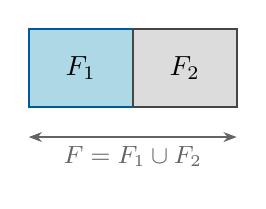
\begin{tikzpicture}[scale=1.1]
  % Additivlik: ikki qo'shni to'rtburchak
  \draw[shapeA] (0,0) rectangle (1.2,0.9) node[midway] {$F_1$};
  \draw[shapeB] (1.2,0) rectangle (2.4,0.9) node[midway] {$F_2$};
  \draw[dimline] (0,-0.35) -- (2.4,-0.35)
    node[midway, below, dimlinelabel] {$F = F_1\cup F_2$};
  \node[below=9pt] at (1.2,-0.35) {};
\end{tikzpicture}
\caption{Additivlik aksiomasi: $\Area{F}=\Area{F_1}+\Area{F_2}$}
\end{subfigure}
\hfill
\begin{subfigure}[b]{0.45\textwidth}
\centering
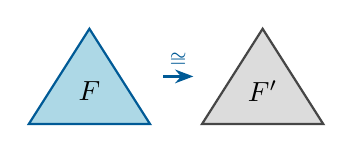
\begin{tikzpicture}[scale=1.1]
  % Invariantlik: kongruent uchburchaklar
  \draw[shapeA] (0,0) -- (1.4,0) -- (0.7,1.1) -- cycle;
  \node at (0.7,0.38) {$F$};
  \draw[shapeB] (2.0,0) -- (3.4,0) -- (2.7,1.1) -- cycle;
  \node at (2.7,0.38) {$F'$};
  \draw[-Stealth, thick, geomblue] (1.55,0.55) -- (1.9,0.55)
    node[midway, above, font=\scriptsize] {$\cong$};
\end{tikzpicture}
\caption{Invariantlik aksiomasi: $\Area{F'}=\Area{F}$}
\end{subfigure}
\caption{Yuza funksiyasining asosiy xossalari}
\label{fig:axioms}
\end{figure}

\begin{lemma}[Monotonlik]
\label{lem:mono}
Agar $F_1 \subseteq F_2$, u holda $\Area{F_1} \le \Area{F_2}$.
\end{lemma}
\begin{proof}
$F_2 = F_1 \cup (F_2 \setminus F_1)$ va ikkala qism ichki nuqtalari bo'yicha
disjunktdir. Additivlik aksiomasi (\ref{ax:add}) va manfiymaslik aksiomasi
(\ref{ax:nonneg}) bo'yicha:
\[
  \Area{F_2} = \Area{F_1} + \Area{F_2\setminus F_1} \ge \Area{F_1}. \qedhere
\]
\end{proof}

\begin{lemma}[Siqish printsipi]
\label{lem:squeeze}
Agar $F_1 \subseteq F \subseteq F_2$ va $\Area{F_2} - \Area{F_1} < \eps$
har qanday $\eps > 0$ uchun bajarilsa, u holda $\Area{F}$ yagona qiymatga ega
bo'lib, u $\Area{F_1} = \Area{F_2}$ ga teng.
\end{lemma}
\begin{proof}
Lemma~\ref{lem:mono} dan $\Area{F_1} \le \Area{F} \le \Area{F_2}$ kelib chiqadi.
Shart bo'yicha $\Area{F_2} - \Area{F_1} < \eps$ har qanday $\eps>0$ uchun
bajariladi, demak $\Area{F_2} = \Area{F_1}$, va shuning uchun
$\Area{F} = \Area{F_1} = \Area{F_2}$.
\end{proof}

% ============================================================
\section{Kvadrat yuzasi}
\label{sec:square}
% ============================================================

\subsection{Tomonining uzunligi \texorpdfstring{$1$}{1} bo'lgan kvadrat}
\label{subsec:sq1}

\begin{aksioma}[Normallashtirish, takrorlash]
Tomoni $1\,\text{m}$ bo'lgan $Q_1$ kvadratning yuzasi $\Area{Q_1}=1\,\text{m}^2$
deb qabul qilinadi.
\end{aksioma}

Bu \emph{ta'rif} ekanligini ta'kidlash lozim: o'lchov birligi shunday tanlanganki,
birlik kvadrat aynan birlik yuzaga ega bo'lsin.

\subsection{Tomonining uzunligi \texorpdfstring{$n \in \N$}{n ∈ N} bo'lgan kvadrat}
\label{subsec:sqn}

\begin{teorema}
\label{thm:sq_nat}
Tomoni $n$ birlik bo'lgan $Q_n$ kvadratning yuzasi $\Area{Q_n} = n^2$.
\end{teorema}
\begin{proof}
$Q_n$ ni har bir tomoni $1$ birlik bo'lgan $n^2$ ta kichik kvadratga $n\times n$
setka yordamida bo'lamiz.
Additivlik aksiomasi (\ref{ax:add}) bo'yicha:
\[
  \Area{Q_n} = \sum_{i=1}^{n^2} \Area{Q_1} = n^2 \cdot 1 = n^2.
\]
\end{proof}

\begin{figure}[h]
\centering
\begin{subfigure}[b]{0.30\textwidth}
\centering
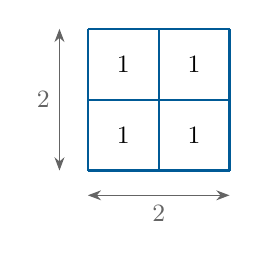
\begin{tikzpicture}[scale=0.9]
  \draw[shapeA, step=1] (0,0) grid (2,2);
  \foreach \x in {0.5,1.5} \foreach \y in {0.5,1.5}
    \node[lab] at (\x,\y) {$1$};
  \draw[dimline] (-0.4,0) -- (-0.4,2) node[midway,left,dimlinelabel] {$2$};
  \draw[dimline] (0,-0.35) -- (2,-0.35) node[midway,below,dimlinelabel] {$2$};
\end{tikzpicture}
\caption{$n=2$: $4$ birlik kvadrat}
\end{subfigure}
\hfill
\begin{subfigure}[b]{0.60\textwidth}
\centering
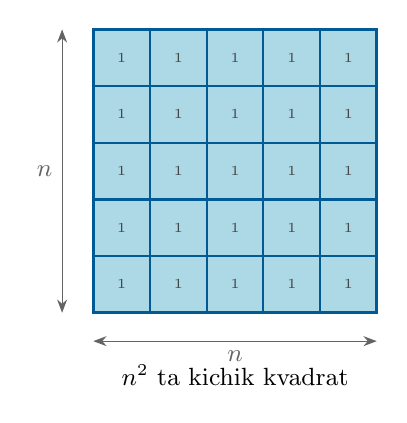
\begin{tikzpicture}[scale=0.72]
  % 5x5 setka
  \fill[fillA] (0,0) rectangle (5,5);
  \draw[step=1, geomblue, thick] (0,0) grid (5,5);
  \draw[geomblue, very thick] (0,0) rectangle (5,5);
  % markerlar
  \foreach \x in {0.5,1.5,2.5,3.5,4.5}
    \foreach \y in {0.5,1.5,2.5,3.5,4.5}
      \node[font=\tiny, geomgray] at (\x,\y) {$1$};
  \draw[dimline] (-0.55,0) -- (-0.55,5) node[midway,left,dimlinelabel] {$n$};
  \draw[dimline] (0,-0.5) -- (5,-0.5) node[midway,below,dimlinelabel] {$n$};
  \node[font=\small] at (2.5,-1.1) {$n^2$ ta kichik kvadrat};
\end{tikzpicture}
\caption{$n=5$ ko'rinishi ($n\times n$ setka)}
\end{subfigure}
\caption{Teorema~\ref{thm:sq_nat}: $\Area{Q_n}=n^2$}
\label{fig:sq_nat}
\end{figure}

\subsection{Tomonining uzunligi \texorpdfstring{$a \in \Qplus$}{a ∈ Q+} bo'lgan kvadrat}
\label{subsec:sqq}

\begin{teorema}
\label{thm:sq_rat}
Tomoni $a \in \Qplus$ bo'lgan $Q_a$ kvadratning yuzasi $\Area{Q_a} = a^2$.
\end{teorema}
\begin{proof}
Har qanday $a\in\Qplus$ uchun musbat butun $n$ va natural $k$ mavjud bo'lib,
$a = n\cdot 10^{-k}$ bo'ladi.

\textbf{1-qadam.} Birlik kvadrat $Q_1$ ni $10^k \times 10^k = 10^{2k}$ ta
mikro-kvadratga bo'lamiz; har bir mikro-kvadratning tomoni $10^{-k}$ va yuzasi
(Teorema~\ref{thm:sq_nat} va proporsionallik) bo'yicha $10^{-2k}$ bo'ladi.

\textbf{2-qadam.} $Q_a$ kvadrat ($Q_1$ ichiga joylashtirilganda) aynan
$n \times n = n^2$ ta mikro-kvadratdan iborat.

\textbf{3-qadam.} Additivlik aksiomasi bo'yicha:
\[
  \Area{Q_a} = n^2 \cdot 10^{-2k} = (n \cdot 10^{-k})^2 = a^2. \qedhere
\]
\end{proof}

\begin{figure}[h]
\centering
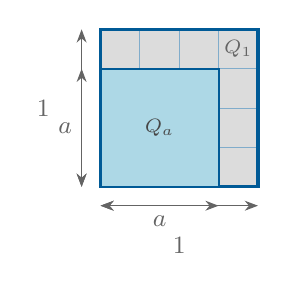
\begin{tikzpicture}[scale=2.0]
  % Birlik kvadrat
  \fill[fillB] (0,0) rectangle (1,1);
  \draw[step=0.25, geomblue!50, thin] (0,0) grid (1,1);
  \draw[geomblue, very thick] (0,0) rectangle (1,1);
  % Q_a = 3/4 ko'rsatish uchun: a = 3*10^{-1}, n=3, k=1 => 10x10 setka
  % Oddiy misol: a = 0.6, n=3, k=1 => setka 10x10 => Q_a = 6x6 birlik?
  % Aslida a=n*10^{-k}: n=3, k=1 => a=0.3
  \fill[fillA] (0,0) rectangle (0.75,0.75);
  \draw[geomblue, thick] (0,0) rectangle (0.75,0.75);
  % etiketlar
  \draw[dimline] (0,-0.12) -- (0.75,-0.12) node[midway,below,dimlinelabel] {$a$};
  \draw[dimline] (0,-0.12) -- (1,-0.12) node[midway,below=8pt,dimlinelabel] {$1$};
  \draw[dimline] (-0.12,0) -- (-0.12,0.75) node[midway,left,dimlinelabel] {$a$};
  \draw[dimline] (-0.12,0) -- (-0.12,1) node[midway,left=8pt,dimlinelabel] {$1$};
  % mikro-setka izohi
  \node[font=\scriptsize, geomgray] at (0.375,0.375) {$Q_a$};
  \node[font=\scriptsize, dimclr] at (0.875,0.875) {$Q_1$};
\end{tikzpicture}
\caption{$Q_a \subset Q_1$: mikro-setka bo'linishi ($a\in\Qplus$)}
\label{fig:sq_rat}
\end{figure}

\subsection{Tomonining uzunligi \texorpdfstring{$x \in \Rplus$}{x ∈ R+} bo'lgan kvadrat}
\label{subsec:sqr}

\begin{teorema}
\label{thm:sq_real}
Tomoni $x \in \Rplus$ bo'lgan $Q_x$ kvadratning yuzasi $\Area{Q_x} = x^2$.
\end{teorema}
\begin{proof}
$x = a + \eps$ deb yozamiz, bu yerda $a \in \Qplus$, $0 \le \eps < 1$.

\textbf{Siqish.} $Q_a \subseteq Q_x \subseteq Q_{a+\eps}$ bo'lishidan
Lemma~\ref{lem:mono} bo'yicha:
\[
  a^2 \;\le\; \Area{Q_x} \;\le\; (a+\eps)^2.
\]
$\eps \to 0$ bo'lganda $a \to x$ va $(a+\eps)^2 \to x^2$.
Siqish printsipi (Lemma~\ref{lem:squeeze}) bo'yicha:
\[
  \Area{Q_x} = x^2. \qedhere
\]
\end{proof}

\begin{figure}[h]
\centering
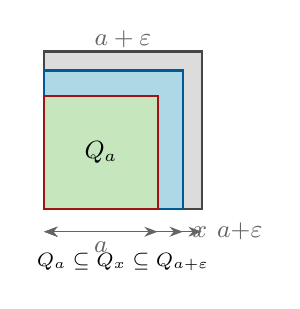
\begin{tikzpicture}[scale=1.6]
  % Tashqi kvadrat Q_{a+eps}
  \fill[fillB] (0,0) rectangle (1.25,1.25);
  \draw[geomgray, thick] (0,0) rectangle (1.25,1.25);
  \node[lab, dimclr] at (0.625, 1.35) {$a+\eps$};
  % Q_x
  \fill[fillA] (0,0) rectangle (1.1,1.1);
  \draw[geomblue, thick] (0,0) rectangle (1.1,1.1);
  \node[lab] at (0.55,0.55) {$Q_x$};
  % Q_a
  \fill[fillC] (0,0) rectangle (0.9,0.9);
  \draw[accred, thick] (0,0) rectangle (0.9,0.9);
  \node[lab] at (0.45,0.45) {$Q_a$};
  % Etiketlar
  \draw[dimline] (0,-0.18) -- (0.9,-0.18) node[midway,below,dimlinelabel] {$a$};
  \draw[dimline] (0,-0.18) -- (1.1,-0.18) node[right,dimlinelabel] {$x$};
  \draw[dimline] (0,-0.18) -- (1.25,-0.18) node[right=2pt,dimlinelabel] {$a{+}\eps$};
  % iqtibos
  \node[font=\scriptsize, align=center] at (0.625,-0.42)
    {$Q_a \subseteq Q_x \subseteq Q_{a+\eps}$};
\end{tikzpicture}
\caption{Siqish printsipi: uchta kvadrat, $\eps\to 0$}
\label{fig:sq_real}
\end{figure}

\begin{natija}
\label{cor:square}
Har qanday $x\in\Rplus$ uchun $\Area{Q_x} = x^2$.
\end{natija}

% ============================================================
\section{To'rtburchak yuzasi}
\label{sec:rect}
% ============================================================

\begin{teorema}
\label{thm:rect}
Tomonlari $a$ va $b$ bo'lgan $R_{a,b}$ to'rtburchak (tik burchakli)ning yuzasi
$\Area{R_{a,b}} = ab$.
\end{teorema}
\begin{proof}
\textbf{Geometrik yasash.}
$a\times b$ to'rtburchakni quyidagi tarzda $(a+b)$ tomonli kvadrat ichiga joylashtiramiz:
\begin{enumerate}[leftmargin=*, label=\textit{Qadam \arabic*}.]
  \item Har bir $a$ tomonning davomiga $b$ uzunlikdagi kesmani qo'shamiz.
  \item Har bir $b$ tomonning davomiga $a$ uzunlikdagi kesmani qo'shamiz.
  \item Hosil bo'lgan to'rtta bo'sh qismni yopamiz — natijada $Q_{a+b}$
        kvadrat hosil bo'ladi.
\end{enumerate}

\textbf{Algebraik munosabat.} $Q_{a+b}$ kvadrat to'rtta qismga bo'lingan
(2.4-rasm): $Q_a$, $Q_b$ va ikkita kongruent $R_{a,b}$ to'rtburchak.
Additivlik va invariantlik aksiomalari bo'yicha:
\[
  \Area{Q_{a+b}} = \Area{Q_a} + \Area{Q_b} + 2\,\Area{R_{a,b}}.
\]
Natija~\ref{cor:square} dan $\Area{Q_{a+b}} = (a+b)^2$, $\Area{Q_a}=a^2$,
$\Area{Q_b}=b^2$. Demak:
\[
  (a+b)^2 = a^2 + b^2 + 2\,\Area{R_{a,b}},
\]
\[
  2\,\Area{R_{a,b}} = (a+b)^2 - a^2 - b^2 = 2ab,
\]
\[
  \Area{R_{a,b}} = ab. \qedhere
\]
\end{proof}

\begin{figure}[h]
\centering
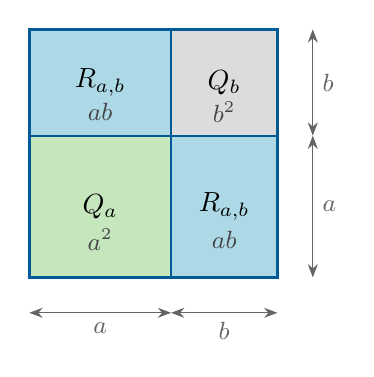
\begin{tikzpicture}[scale=1.5]
  % (a+b) x (a+b) kvadrat, a=1.2, b=0.9
  \pgfmathsetmacro{\a}{1.2}
  \pgfmathsetmacro{\b}{0.9}
  \pgfmathsetmacro{\s}{\a+\b}
  % Q_a (pastki chap)
  \fill[fillC] (0,0) rectangle (\a,\a);
  \draw[geomblue,thick] (0,0) rectangle (\a,\a);
  \node at (\a/2, \a/2) {$Q_a$};
  \node[font=\small, geomgray] at (\a/2, \a/2-0.28) {$a^2$};
  % Q_b (yuqori o'ng)
  \fill[fillB] (\a,\a) rectangle (\s,\s);
  \draw[geomblue,thick] (\a,\a) rectangle (\s,\s);
  \node at (\a+\b/2, \a+\b/2) {$Q_b$};
  \node[font=\small, geomgray] at (\a+\b/2, \a+\b/2-0.25) {$b^2$};
  % R_{a,b} (pastki o'ng)
  \fill[fillA] (\a,0) rectangle (\s,\a);
  \draw[geomblue,thick] (\a,0) rectangle (\s,\a);
  \node at (\a+\b/2, \a/2) {$R_{a,b}$};
  \node[font=\small, geomgray] at (\a+\b/2, \a/2-0.28) {$ab$};
  % R_{a,b} (yuqori chap)
  \fill[fillA] (0,\a) rectangle (\a,\s);
  \draw[geomblue,thick] (0,\a) rectangle (\a,\s);
  \node at (\a/2, \a+\b/2) {$R_{a,b}$};
  \node[font=\small, geomgray] at (\a/2, \a+\b/2-0.25) {$ab$};
  % tashqi kvadrat konturi
  \draw[geomblue, very thick] (0,0) rectangle (\s,\s);
  % O'lchov chiziqlari
  \draw[dimline] (0,-0.3) -- (\a,-0.3) node[midway,below,dimlinelabel] {$a$};
  \draw[dimline] (\a,-0.3) -- (\s,-0.3) node[midway,below,dimlinelabel] {$b$};
  \draw[dimline] (\s+0.3,0) -- (\s+0.3,\a) node[midway,right,dimlinelabel] {$a$};
  \draw[dimline] (\s+0.3,\a) -- (\s+0.3,\s) node[midway,right,dimlinelabel] {$b$};
\end{tikzpicture}
\caption{$(a+b)\times(a+b)$ kvadrat: $Q_a$, $Q_b$ va ikkita $R_{a,b}$}
\label{fig:rect}
\end{figure}

% ============================================================
\section{To'g'ri burchakli uchburchak yuzasi}
\label{sec:righttri}
% ============================================================

\begin{teorema}
\label{thm:righttri}
Katetlari $a$ va $b$ bo'lgan to'g'ri burchakli $T_{a,b}$ uchburchak yuzasi
$\displaystyle\Area{T_{a,b}} = \frac{ab}{2}$.
\end{teorema}
\begin{proof}
$R_{a,b}$ to'rtburchakka diagonal $BD$ tortamiz
(5-rasm: $A=(0,0)$, $B=(a,0)$, $C=(a,b)$, $D=(0,b)$).
Diagonal $R_{a,b}$ ni ikkita uchburchakka $T_1 = ABD$ va $T_2 = BCD$ ga ajratadi.

$T_1$ va $T_2$ birining ustiga ikkinchisini $BC$ bo'ylab aks ettirganda mos tushadi;
demak invariantlik aksiomasi bo'yicha $\Area{T_1} = \Area{T_2}$.

Additivlik aksiomasi bo'yicha:
\[
  \Area{R_{a,b}} = \Area{T_1} + \Area{T_2} = 2\,\Area{T_1}.
\]
Teorema~\ref{thm:rect} dan $\Area{R_{a,b}} = ab$, shuning uchun:
\[
  \Area{T_{a,b}} = \Area{T_1} = \frac{ab}{2}. \qedhere
\]
\end{proof}

\begin{figure}[h]
\centering
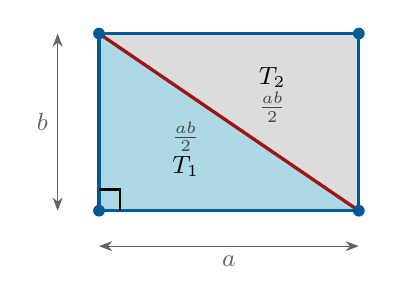
\begin{tikzpicture}[scale=1.5]
  \pgfmathsetmacro{\a}{2.2}
  \pgfmathsetmacro{\b}{1.5}
  % To'liq to'rtburchak
  \fill[fillB!50] (0,0) rectangle (\a,\b);
  % T1 — pastki uchburchak (ko'k)
  \fill[fillA] (0,0) -- (\a,0) -- (0,\b) -- cycle;
  % T2 — yuqori uchburchak (kulrang)
  \fill[fillB] (\a,0) -- (\a,\b) -- (0,\b) -- cycle;
  % Konturlar
  \draw[geomblue, very thick] (0,0) rectangle (\a,\b);
  \draw[accred, very thick] (0,\b) -- (\a,0);
  % Etiketlar
  \node[lab] at (\a/3, \b/4) {$T_1$};
  \node[font=\small, geomgray] at (\a/3, \b/4+0.25) {$\tfrac{ab}{2}$};
  \node[lab] at (2*\a/3, 3*\b/4) {$T_2$};
  \node[font=\small, geomgray] at (2*\a/3, 3*\b/4-0.25) {$\tfrac{ab}{2}$};
  % Burchak belgilari
  \draw[thick] (0,0.18) -- (0.18,0.18) -- (0.18,0);
  % O'lchov chiziqlari
  \draw[dimline] (0,-0.3) -- (\a,-0.3) node[midway,below,dimlinelabel] {$a$};
  \draw[dimline] (-0.35,0) -- (-0.35,\b) node[midway,left,dimlinelabel] {$b$};
  % Burchaklar
  \node[dotpt] at (0,0) {};
  \node[dotpt] at (\a,0) {};
  \node[dotpt] at (\a,\b) {};
  \node[dotpt] at (0,\b) {};
\end{tikzpicture}
\caption{Diagonal to'rtburchakni ikkita kongruent to'g'ri burchakli uchburchakka
         bo'ladi; har birining yuzasi $\tfrac{ab}{2}$}
\label{fig:righttri}
\end{figure}

% ============================================================
\section{Ixtiyoriy uchburchak yuzasi}
\label{sec:tri}
% ============================================================

\begin{teorema}
\label{thm:tri}
$ABC$ uchburchakda $c = |AB|$ va $h_c$ — $C$ uchidan $AB$ ga tushirilgan
balandlik bo'lsa, u holda
\[
  \Area{ABC} = \frac{1}{2}\,c\,h_c.
\]
\end{teorema}
\begin{proof}
$D$ — balandlik asosi ($CD \perp AB$, $D \in AB$ yoki uning davomi).

\textbf{Holat 1: $D$ ichki nuqtada} (qur yoki o'tmas uchburchak).
$AD = x$, $DB = c - x$.
Additivlik aksiomasi bo'yicha:
\[
  \Area{ABC} = \Area{ACD} + \Area{BCD}
    = \frac{1}{2}\,x\,h_c + \frac{1}{2}(c-x)\,h_c
    = \frac{1}{2}\,c\,h_c.
\]

\textbf{Holat 2: $D$ tashqi nuqtada} (o'tmas burchak $A$ yoki $B$ da).
Masalan, $D$ ning $B$ dan tashqarida, ya'ni $AD = x > c$ deb faraz qilaylik.
\[
  \Area{ABD} = \Area{ACD} - \Area{BCD}
    = \frac{1}{2}\,x\,h_c - \frac{1}{2}(x-c)\,h_c = \frac{1}{2}\,c\,h_c.
\]
Ikkala holda ham natija bir xil. \qedhere
\end{proof}

\begin{figure}[h]
\centering
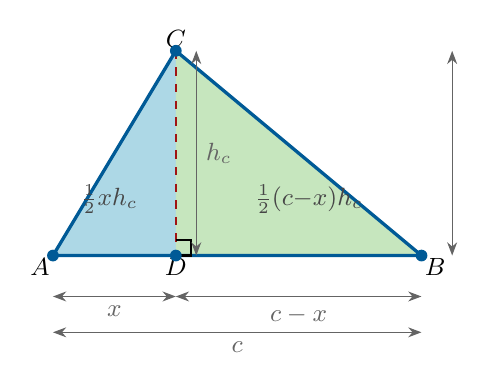
\begin{tikzpicture}[scale=1.3]
  % Vertices
  \coordinate (A) at (0,0);
  \coordinate (B) at (3.6,0);
  \coordinate (C) at (1.2,2.0);
  \coordinate (D) at (1.2,0); % balandlik asosi
  % To'ldirishlar
  \fill[fillA] (A) -- (D) -- (C) -- cycle;
  \fill[fillC] (D) -- (B) -- (C) -- cycle;
  % Konturlar
  \draw[geomblue, very thick] (A) -- (B) -- (C) -- cycle;
  % Balandlik
  \draw[accred, thick, dashed] (C) -- (D);
  \draw[thick] (D) -- ++(0.15,0) -- ++(0,0.15) -- ++(-0.15,0);
  % Etiketlar
  \node[below left,lab] at (A) {$A$};
  \node[below right,lab] at (B) {$B$};
  \node[above,lab] at (C) {$C$};
  \node[below,lab] at (D) {$D$};
  % O'lchov chiziqlari
  \draw[dimline] (0,-0.4) -- (1.2,-0.4) node[midway,below,dimlinelabel] {$x$};
  \draw[dimline] (1.2,-0.4) -- (3.6,-0.4) node[midway,below,dimlinelabel] {$c-x$};
  \draw[dimline] (3.9,0) -- (3.9,2.0) node[midway,right,dimlinelabel] {};
  \draw[dimline] (1.4,0) -- (1.4,2.0) node[midway,right,dimlinelabel] {$h_c$};
  % yuza etiketlari
  \node[lab, geomgray] at (0.55,0.55) {$\tfrac{1}{2}xh_c$};
  \node[lab, geomgray] at (2.5,0.55) {$\tfrac{1}{2}(c{-}x)h_c$};
  % c etiket
  \draw[dimline] (0,-0.75) -- (3.6,-0.75) node[midway,below,dimlinelabel] {$c$};
  \node[dotpt] at (A) {};
  \node[dotpt] at (B) {};
  \node[dotpt] at (C) {};
  \node[dotpt] at (D) {};
\end{tikzpicture}
\caption{Balandlik $h_c$ orqali ixtiyoriy uchburchak yuzasi}
\label{fig:tri}
\end{figure}

\subsection{Trigonometrik ko'rinish}
\label{subsec:trig}

\begin{teorema}
\label{thm:tri_trig}
$ABC$ uchburchakda $a = BC$, $b = CA$, $c = AB$ va $\alpha,\beta,\gamma$ —
mos burchaklar bo'lsa:
\[
  \Area{ABC}
    = \frac{1}{2}\,ca\sin\alpha
    = \frac{1}{2}\,cb\sin\beta
    = \frac{1}{2}\,ab\sin\gamma.
\]
\end{teorema}
\begin{proof}
$C$ uchidan tushirilgan balandlik $h_c = a\sin\alpha = b\sin\beta$ bo'ladi
(to'g'ri burchakli uchburchak ta'rifidan).
Teorema~\ref{thm:tri} bo'yicha:
\[
  \Area{ABC} = \tfrac{1}{2}\,c\,h_c = \tfrac{1}{2}\,c\,a\sin\alpha
    = \tfrac{1}{2}\,c\,b\sin\beta.
\]
$A$ uchidan tushirilgan balandlik $h_a = b\sin\gamma$ bo'lgani uchun
$\Area{ABC} = \tfrac{1}{2}\,a\,h_a = \tfrac{1}{2}\,ab\sin\gamma$. \qedhere
\end{proof}

\begin{formulabox}[Uchburchak yuzasining to'rtta ekvivalent ko'rinishi]
\[
  \Area{ABC} = \frac{1}{2}\,c\,h_c
             = \frac{1}{2}\,ca\sin\alpha
             = \frac{1}{2}\,cb\sin\beta
             = \frac{1}{2}\,ab\sin\gamma
\]
\end{formulabox}

% ============================================================
\section{Parallelogramm yuzasi}
\label{sec:para}
% ============================================================

\begin{teorema}
\label{thm:para}
Asosi $a$ va balandligi $h$ bo'lgan $ABCD$ parallelogrammning yuzasi
$\Area{ABCD} = a\,h$.
\end{teorema}
\begin{proof}
$E$ — $D$ dan $AB$ ga tushirilgan balandlik asosi; $F$ — $C$ dan $AB$ ga
tushirilgan balandlik asosi.
$DEFC$ to'rtburchak $a \times h$ o'lchamli to'rtburchakdir.

$\triangle AED \cong \triangle BFC$ (ikkita katetlari teng: $DE=CF=h$,
$AD=BC$), shu sababli invariantlik aksiomasi bo'yicha ularning yuzalari teng.

Additivlik bo'yicha:
\[
  \Area{ABCD}
    = \Area{AEFD} + \Area{AED}
      \quad\text{(yoki)}
    = \Area{BEFC} - \Area{BFC} + \Area{AED}.
\]
Ikkita kongruent uchburchakni almashtirish (``kesib-qo'yish'' usuli) natijasida:
\[
  \Area{ABCD} = \Area{R_{a,h}} = a\,h. \qedhere
\]
\end{proof}

\begin{figure}[h]
\centering
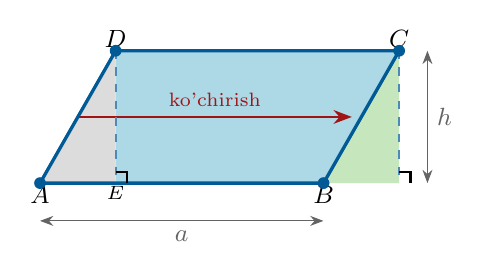
\begin{tikzpicture}[scale=1.2]
  % Parallelogramm ABCD
  \coordinate (A) at (0,0);
  \coordinate (B) at (3,0);
  \coordinate (C) at (3.8,1.4);
  \coordinate (D) at (0.8,1.4);
  \coordinate (E) at (0.8,0);  % D dan tushirilgan balandlik
  \coordinate (F) at (3.8,0);  % C dan tushirilgan balandlik (to'rtburchak tashqarida)
  % Parallelogramm asosiy qismi (to'rtburchak: EBCF yoki E,B,C,D qism)
  \fill[fillA] (E) -- (B) -- (C) -- (D) -- cycle;
  % O'ngdan kesma uchburchak BFC (qo'shilish uchun)
  \fill[fillC] (B) -- (F) -- (C) -- cycle;
  % Chapdan kesma uchburchak AED
  \fill[fillB] (A) -- (E) -- (D) -- cycle;
  % Ko'rsatish uchun o'q (kesib ko'chirish)
  \draw[-Stealth, thick, accred] (0.4,0.7) -- ++(2.9,0)
    node[midway, above, font=\scriptsize, accred] {ko'chirish};
  % Konturlar
  \draw[geomblue, very thick] (A) -- (B) -- (C) -- (D) -- cycle;
  \draw[geomdash] (D) -- (E);
  \draw[geomdash] (C) -- (F);
  \draw[thick] (E) ++(0.12,0) -- ++(0,0.12) -- ++(-0.12,0);
  \draw[thick] (F) ++(0.12,0) -- ++(0,0.12) -- ++(-0.12,0);
  % Etiketlar
  \node[below,lab] at (A) {$A$};
  \node[below,lab] at (B) {$B$};
  \node[above,lab] at (C) {$C$};
  \node[above,lab] at (D) {$D$};
  \node[below,lab, font=\scriptsize] at (E) {$E$};
  % O'lchov chiziqlari
  \draw[dimline] (0,-0.4) -- (3,-0.4) node[midway,below,dimlinelabel] {$a$};
  \draw[dimline] (3.8+0.3,0) -- (3.8+0.3,1.4) node[midway,right,dimlinelabel] {$h$};
  \node[dotpt] at (A) {};
  \node[dotpt] at (B) {};
  \node[dotpt] at (C) {};
  \node[dotpt] at (D) {};
\end{tikzpicture}
\caption{Parallelogramm: chap uchburchakni o'ngga ko'chirish --- $a\times h$ to'rtburchak hosil bo'ladi}
\label{fig:para}
\end{figure}

\subsection{Romb yuzasi}
\label{subsec:rhombus}

\begin{teorema}
\label{thm:rhombus}
Diagonallari $d_1$ va $d_2$ bo'lgan $ABCD$ rombning yuzasi
$\displaystyle\Area{ABCD} = \frac{d_1 d_2}{2}$.
\end{teorema}
\begin{proof}
Rombning diagonallari bir-birini perpendikulyar va tenglamasdan kesishadi;
kesishish nuqtasi $O$ bo'lsin.
$O$ har bir diagonalni ikki teng qismga bo'ladi:
$AO=OC=\tfrac{d_1}{2}$, $BO=OD=\tfrac{d_2}{2}$.

Diagonallar to'rtta kongruent to'g'ri burchakli uchburchakka $T_1,T_2,T_3,T_4$
bo'ladi; har birining katetlari $\tfrac{d_1}{2}$ va $\tfrac{d_2}{2}$, shuning
uchun
\[
  \Area{T_i} = \frac{1}{2}\cdot\frac{d_1}{2}\cdot\frac{d_2}{2}
             = \frac{d_1 d_2}{8}.
\]
Additivlik bo'yicha:
\[
  \Area{ABCD} = 4\cdot\frac{d_1 d_2}{8} = \frac{d_1 d_2}{2}. \qedhere
\]
\end{proof}

\begin{figure}[h]
\centering
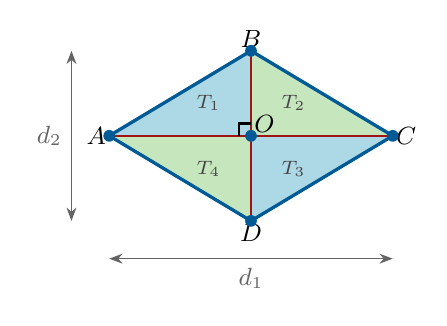
\begin{tikzpicture}[scale=1.2]
  \coordinate (A) at (-1.5,0);
  \coordinate (B) at (0,0.9);
  \coordinate (C) at (1.5,0);
  \coordinate (D) at (0,-0.9);
  \coordinate (O) at (0,0);
  % To'ldirishlar
  \fill[fillA] (A) -- (B) -- (O) -- cycle;
  \fill[fillC] (B) -- (C) -- (O) -- cycle;
  \fill[fillA] (C) -- (D) -- (O) -- cycle;
  \fill[fillC] (D) -- (A) -- (O) -- cycle;
  % Konturlar
  \draw[geomblue, very thick] (A) -- (B) -- (C) -- (D) -- cycle;
  \draw[accred, thick] (A) -- (C);
  \draw[accred, thick] (B) -- (D);
  % O'ng burchak belgilari
  \draw[thick] (-0.13,0) -- (-0.13,0.13) -- (0,0.13);
  % Etiketlar
  \node[left,lab] at (A) {$A$};
  \node[above,lab] at (B) {$B$};
  \node[right,lab] at (C) {$C$};
  \node[below,lab] at (D) {$D$};
  \node[above right, font=\scriptsize,lab] at (O) {$O$};
  % Yuza etiketlari
  \node[font=\scriptsize,geomgray] at (-0.45,0.35) {$T_1$};
  \node[font=\scriptsize,geomgray] at (0.45,0.35) {$T_2$};
  \node[font=\scriptsize,geomgray] at (0.45,-0.35) {$T_3$};
  \node[font=\scriptsize,geomgray] at (-0.45,-0.35) {$T_4$};
  % O'lchov chiziqlari
  \draw[dimline] (-1.5,-1.3) -- (1.5,-1.3) node[midway,below,dimlinelabel] {$d_1$};
  \draw[dimline] (-1.9,-0.9) -- (-1.9,0.9) node[midway,left,dimlinelabel] {$d_2$};
  \foreach \pt in {A,B,C,D,O} \node[dotpt] at (\pt) {};
\end{tikzpicture}
\caption{Romb: ikkita diagonali to'rtta kongruent to'g'ri burchakli uchburchakka bo'ladi}
\label{fig:rhombus}
\end{figure}

\subsection{Trapetsiya yuzasi}
\label{subsec:trap}

\begin{teorema}
\label{thm:trap}
Asoslari $a$ va $b$ ($a>b$) va balandligi $h$ bo'lgan $ABCD$ trapetsiyaning yuzasi
$\displaystyle\Area{ABCD} = \frac{(a+b)\,h}{2}$.
\end{teorema}
\begin{proof}
Ikkita kongruent trapetsiya olamiz: asl $ABCD$ va uning $180^\circ$ ga aylantirilgan
nusxasi $A'B'C'D'$.
$CD$ va $C'D'$ tomonlarini tutashtiramiz — natijada asosi $a+b$ va balandligi $h$
bo'lgan parallelogramm hosil bo'ladi.

Teorema~\ref{thm:para} bo'yicha:
\[
  \Area{\text{parallelogramm}} = (a+b)\,h.
\]
Additivlik va invariantlik bo'yicha:
\[
  \Area{ABCD} = \frac{(a+b)\,h}{2}. \qedhere
\]
\end{proof}

\begin{figure}[h]
\centering
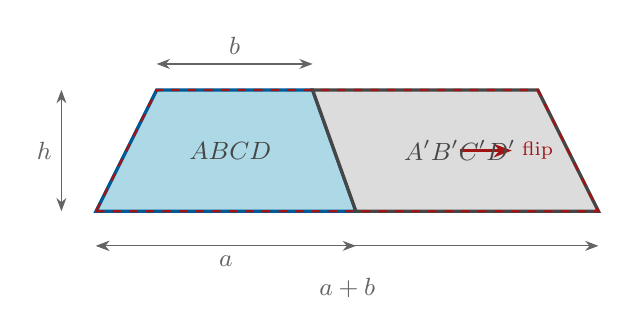
\begin{tikzpicture}[scale=1.1]
  % Trapetsiya: a=3, b=1.6, h=1.4
  % Asl trapetsiya (to'q ko'k)
  \fill[fillA] (0,0) -- (3,0) -- (2.5,1.4) -- (0.7,1.4) -- cycle;
  \draw[geomblue, very thick] (0,0) -- (3,0) -- (2.5,1.4) -- (0.7,1.4) -- cycle;
  % Teskari trapetsiya (kulrang), to'g'ri yopishtiriladi
  \fill[fillB] (3,0) -- (5.8,0) -- (5.1,1.4) -- (2.5,1.4) -- cycle;
  \draw[geomgray, very thick] (3,0) -- (5.8,0) -- (5.1,1.4) -- (2.5,1.4) -- cycle;
  % Parallelogramm konturi
  \draw[accred, dashed, thick] (0,0) -- (5.8,0) -- (5.1,1.4) -- (0.7,1.4) -- cycle;
  % Balandlik
  \draw[dimline] (-0.4,0) -- (-0.4,1.4) node[midway,left,dimlinelabel] {$h$};
  % asoslar
  \draw[dimline] (0,-0.4) -- (3,-0.4) node[midway,below,dimlinelabel] {$a$};
  \draw[dimline] (0.7,1.7) -- (2.5,1.7) node[midway,above,dimlinelabel] {$b$};
  \draw[dimline] (0,-0.4) -- (5.8,-0.4) node[midway,below=8pt,dimlinelabel] {$a+b$};
  % Ko'chirish o'qi
  \draw[-Stealth, thick, accred] (4.2,0.7) -- ++(0.6,0)
    node[right, font=\scriptsize, accred] {flip};
  % Etiketlar
  \node[font=\small,geomgray] at (1.55,0.7) {$ABCD$};
  \node[font=\small,geomgray] at (4.2,0.7) {$A'B'C'D'$};
\end{tikzpicture}
\caption{Ikkita trapetsiyadan parallelogramm hosil qilish}
\label{fig:trap}
\end{figure}

\subsection{Ixtiyoriy qavariq to'rtburchak yuzasi}
\label{subsec:convex_quad}

\begin{teorema}
\label{thm:convex_quad}
$ABCD$ qavariq to'rtburchak diagonal $AC$ orqali ikkita uchburchakka $ABC$ va
$ACD$ ga bo'linadi; uning yuzasi:
\[
  \Area{ABCD} = \Area{ABC} + \Area{ACD}.
\]
\end{teorema}
\begin{proof}
$ABCD$ qavariq bo'lgani uchun diagonal $AC$ to'rtburchak ichida yotadi.
Additivlik aksiomasi bo'yicha natija to'g'ridan-to'g'ri kelib chiqadi.
$\Area{ABC}$ va $\Area{ACD}$ ni Teorema~\ref{thm:tri} bilan hisoblaymiz. \qedhere
\end{proof}

\begin{figure}[h]
\centering
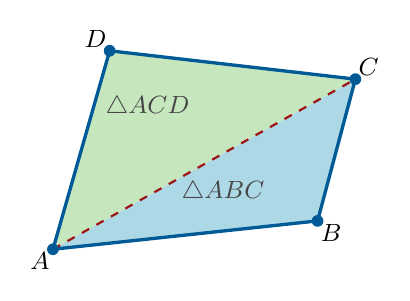
\begin{tikzpicture}[scale=1.2]
  \coordinate (A) at (0,0);
  \coordinate (B) at (2.8,0.3);
  \coordinate (C) at (3.2,1.8);
  \coordinate (D) at (0.6,2.1);
  % To'ldirishlar
  \fill[fillA] (A) -- (B) -- (C) -- cycle;
  \fill[fillC] (A) -- (C) -- (D) -- cycle;
  % Konturlar
  \draw[geomblue, very thick] (A) -- (B) -- (C) -- (D) -- cycle;
  \draw[accred, thick, dashed] (A) -- (C);
  % Etiketlar
  \node[below left,lab] at (A) {$A$};
  \node[below right,lab] at (B) {$B$};
  \node[above right,lab] at (C) {$C$};
  \node[above left,lab] at (D) {$D$};
  \node[lab, geomgray] at (1.8,0.6) {$\triangle ABC$};
  \node[lab, geomgray] at (1.0,1.5) {$\triangle ACD$};
  \foreach \pt in {A,B,C,D} \node[dotpt] at (\pt) {};
\end{tikzpicture}
\caption{Qavariq to'rtburchak: diagonal $AC$ orqali ikkita uchburchakka bo'linadi}
\label{fig:convex_quad}
\end{figure}

% ============================================================
\section{Qavariq ko'pburchak yuzasi}
\label{sec:polygon}
% ============================================================

\begin{teorema}[Triangulyatsiya {\cite{Coxeter1969}}]
\label{thm:polygon}
$n$ ta uchli $P_n = A_1 A_2 \cdots A_n$ qavariq ko'pburchak $A_1$ uchidan
chizilgan $(n-3)$ ta diagonal bilan $(n-2)$ ta uchburchakka:
$T_k = A_1 A_{k+1} A_{k+2}$, $k=1,\ldots,n-2$, bo'linadi va
\[
  \Area{P_n} = \sum_{k=1}^{n-2} \Area{A_1 A_{k+1} A_{k+2}}.
\]
\end{teorema}
\begin{proof}
Qavariqlik sababli $A_1$dan $A_3, A_4, \ldots, A_{n-1}$ ga chizilgan har bir
diagonal to'liq ko'pburchak ichida yotadi va ular bir-biriga ichki nuqtalarda
kesishmaydi.
Hosil bo'lgan $(n-2)$ ta uchburchak bir-birining ichki nuqtalarsiz qoplab oladi
va yig'ib ko'pburchakni to'ldiradi. Additivlik aksiomasi bilan zudlik bilan
natija kelib chiqadi. \qedhere
\end{proof}

\begin{figure}[h]
\centering
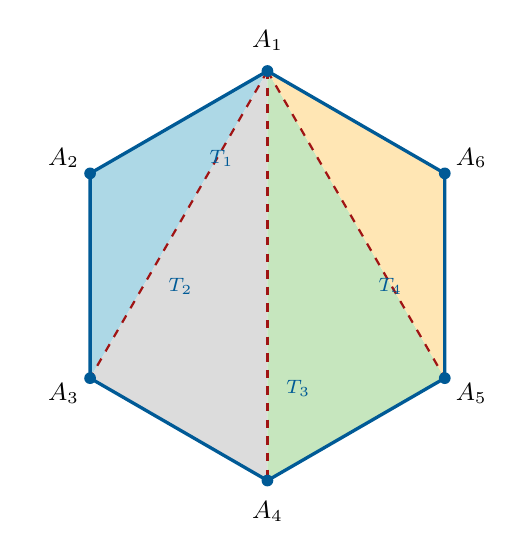
\begin{tikzpicture}[scale=1.3]
  % Olti burchak: n=6
  \def\R{2}
  \foreach \i in {1,...,6}{
    \coordinate (A\i) at ({90+(\i-1)*60}:\R);
  }
  % To'ldirishlar (4 ta uchburchak)
  \fill[fillA] (A1) -- (A2) -- (A3) -- cycle;
  \fill[fillB] (A1) -- (A3) -- (A4) -- cycle;
  \fill[fillC] (A1) -- (A4) -- (A5) -- cycle;
  \fill[fillD] (A1) -- (A5) -- (A6) -- cycle;
  % Konturlar
  \draw[geomblue, very thick] (A1) -- (A2) -- (A3) -- (A4) -- (A5) -- (A6) -- cycle;
  % Diagonallar
  \draw[accred, thick, dashed] (A1) -- (A3);
  \draw[accred, thick, dashed] (A1) -- (A4);
  \draw[accred, thick, dashed] (A1) -- (A5);
  % Etiketlar
  \foreach \i in {1,...,6}{
    \node[lab, font=\small] at ({90+(\i-1)*60}:{\R+0.3}) {$A_{\i}$};
  }
  % Uchburchak nomlari
  \node[font=\scriptsize, geomgray] at ($ (A1)!0.6!(A2) + (A3)!0.3!(A1) - (A1)$) {};
  \node[font=\scriptsize, geomblue] at (-0.45,1.15) {$T_1$};
  \node[font=\scriptsize, geomblue] at (-0.85,-0.1) {$T_2$};
  \node[font=\scriptsize, geomblue] at (0.3,-1.1) {$T_3$};
  \node[font=\scriptsize, geomblue] at (1.2,-0.1) {$T_4$};
  \foreach \i in {1,...,6} \node[dotpt] at (A\i) {};
\end{tikzpicture}
\caption{Olti burchakning $A_1$ uchidan triangulyatsiyasi: $T_1, T_2, T_3, T_4$}
\label{fig:polygon}
\end{figure}

\begin{izoh}
$n=4$ (to'rtburchak): $2$ uchburchak --- Teorema~\ref{thm:convex_quad}ning
maxsus holi. $n=5$ (beshburchak): $3$ uchburchak. $n=6$ (olti burchak):
$4$ uchburchak (14-rasm).
\end{izoh}

% ============================================================
\section{Doira yuzasi}
\label{sec:circle}
% ============================================================

\begin{teorema}
\label{thm:circle}
Radiusi $R$ bo'lgan doiraning yuzasi $\Area{\odot(R)} = \pi R^2$.
\end{teorema}
\begin{proof}
\textbf{Ichki ko'pburchak.}
Radiusi $R$ bo'lgan doiraga ichki chizilgan muntazam $n$-burchak $P_n^{\rm in}$
ni qaraymiz. Uning tomoni $a_n = 2R\sin(\pi/n)$.
Triangulyatsiya (Teorema~\ref{thm:polygon}) va Teorema~\ref{thm:tri_trig} bo'yicha:
\[
  \Area{P_n^{\rm in}} = \frac{n}{2}\,R^2\sin\!\left(\frac{2\pi}{n}\right).
\]

\textbf{Tashqi ko'pburchak.}
Doirani o'rab olgan muntazam $n$-burchak $P_n^{\rm out}$ning yuzasi:
\[
  \Area{P_n^{\rm out}} = n\,R^2\tan\!\left(\frac{\pi}{n}\right).
\]

\textbf{Siqish.}
$P_n^{\rm in} \subseteq \odot(R) \subseteq P_n^{\rm out}$ bo'lgani uchun
Lemma~\ref{lem:mono} va Lemma~\ref{lem:squeeze} bo'yicha:
\[
  \frac{n}{2}\,R^2\sin\!\left(\frac{2\pi}{n}\right)
  \;\le\;
  \Area{\odot(R)}
  \;\le\;
  n\,R^2\tan\!\left(\frac{\pi}{n}\right).
\]

\textbf{Limit.}
$t = \pi/n \to 0$ qo'yib, birinchi ajoyib limitni ($\lim_{t\to 0}\tfrac{\sin t}{t}=1$
va $\lim_{t\to 0}\tfrac{\tan t}{t}=1$) qo'llamiz:
\[
  \frac{n}{2}\,R^2\sin\!\left(\frac{2\pi}{n}\right)
  = \pi R^2 \cdot \frac{\sin(2\pi/n)}{2\pi/n}
  \xrightarrow{n\to\infty} \pi R^2,
\]
\[
  n\,R^2\tan\!\left(\frac{\pi}{n}\right)
  = \pi R^2 \cdot \frac{\tan(\pi/n)}{\pi/n}
  \xrightarrow{n\to\infty} \pi R^2.
\]
Siqish printsipi bo'yicha $\Area{\odot(R)} = \pi R^2$. \qedhere
\end{proof}

\begin{figure}[h]
\centering
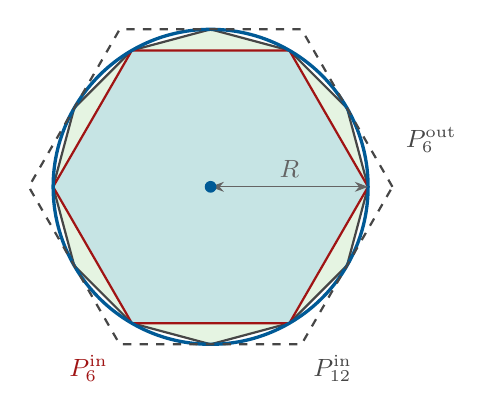
\begin{tikzpicture}[scale=1.0]
  \pgfmathsetmacro{\R}{2}
  \pgfmathsetmacro{\Rout}{\R / cos(30)}  % tashqi heksagon radiusi = R / cos(pi/6)
  % n=12 ichki ko'pburchak (avval, orqa fon)
  \fill[fillC, opacity=0.45]
    (0:\R) -- (30:\R) -- (60:\R) -- (90:\R) -- (120:\R) -- (150:\R) --
    (180:\R) -- (210:\R) -- (240:\R) -- (270:\R) -- (300:\R) -- (330:\R) -- cycle;
  \draw[geomgray, thick]
    (0:\R) -- (30:\R) -- (60:\R) -- (90:\R) -- (120:\R) -- (150:\R) --
    (180:\R) -- (210:\R) -- (240:\R) -- (270:\R) -- (300:\R) -- (330:\R) -- cycle;
  % n=6 ichki heksagon (ustiga)
  \fill[fillA, opacity=0.55]
    (0:\R) -- (60:\R) -- (120:\R) -- (180:\R) -- (240:\R) -- (300:\R) -- cycle;
  \draw[accred, thick]
    (0:\R) -- (60:\R) -- (120:\R) -- (180:\R) -- (240:\R) -- (300:\R) -- cycle;
  % Doira (eng ustida)
  \draw[geomblue, very thick] (0,0) circle (\R);
  % Tashqi heksagon (n=6 tashqi ko'pburchak)
  \draw[geomgray, dashed, thick]
    (0:\Rout) -- (60:\Rout) -- (120:\Rout) -- (180:\Rout) -- (240:\Rout) -- (300:\Rout) -- cycle;
  % Radius
  \draw[dimline] (0,0) -- (\R,0) node[midway, above, dimlinelabel] {$R$};
  \node[dotpt] at (0,0) {};
  % Etiketlar
  \node[font=\small, accred]   at (-1.55, -2.3) {$P_6^{\mathrm{in}}$};
  \node[font=\small, geomgray] at ( 1.55, -2.3) {$P_{12}^{\mathrm{in}}$};
  \node[font=\small, geomgray] at ( 2.8,   0.6) {$P_6^{\mathrm{out}}$};
\end{tikzpicture}
\caption{Ichki ($n=6$, $n=12$) va tashqi ($n=6$) ko'pburchaklar doiraga yaqinlashadi}
\label{fig:circle}
\end{figure}

% ============================================================
\section{Ellips yuzasi}
\label{sec:ellipse}
% ============================================================

\begin{tarif}[Ellips]
\label{def:ellipse}
$E_{a,b} = \bigl\{(x,y)\in\R^2 : \tfrac{x^2}{a^2}+\tfrac{y^2}{b^2}\le 1\bigr\}$
deb aniqlangan chekli to'plam \emph{ellips} deyiladi; $a>0$ va $b>0$ — katta va
kichik yarim o'qlar.
\end{tarif}

\begin{lemma}[Affin o'zgarish va yuza {\cite{Berger1987, Yaglom1961}}]
\label{lem:affine}
$T\colon(u,v)\mapsto(au, bv)$ affin o'zgarishi (cho'zish) har qanday
$F\in\mathcal{F}$ shaklning yuzasini $ab$ martaga oshiradi:
$\Area{T(F)} = ab\cdot\Area{F}$.
\end{lemma}
\begin{proof}
To'rtburchaklar uchun: $a_0\times b_0$ to'rtburchak $T$ ta'sirida
$aa_0 \times bb_0$ to'rtburchakka o'tadi, yuzasi $ab\cdot a_0 b_0 = ab\cdot\Area{R}$.
Ixtiyoriy shakl uchun Lemma~\ref{lem:squeeze} (siqish printsipi) bilan to'rtburchaklar
orqali taqribiy qiymatilab, $\Area{T(F)} = ab\cdot\Area{F}$ keltirib chiqariladi.
\end{proof}

\begin{teorema}
\label{thm:ellipse}
$E_{a,b}$ ellipsning yuzasi $\Area{E_{a,b}} = \pi\,ab$.
\end{teorema}
\begin{proof}
$D = E_{1,1}$ — birlik disk (radiusi $1$ bo'lgan doira).
Teorema~\ref{thm:circle} bo'yicha $\Area{D} = \pi$.

$T\colon(u,v)\mapsto(au,bv)$ affin o'zgarishi $D$ ni $E_{a,b}$ ga o'tkazadi:
\[
  \frac{(au)^2}{a^2}+\frac{(bv)^2}{b^2} = u^2+v^2 \le 1
  \iff (u,v)\in D.
\]
Lemma~\ref{lem:affine} bo'yicha:
\[
  \Area{E_{a,b}} = ab\cdot\Area{D} = \pi\,ab. \qedhere
\]
\end{proof}

\begin{izoh}
$T$ ning Yaqob determinanti $\det\begin{pmatrix}a&0\\0&b\end{pmatrix} = ab$ —
Analiz kursi bilan aloqa.
\end{izoh}

\begin{figure}[h]
\centering
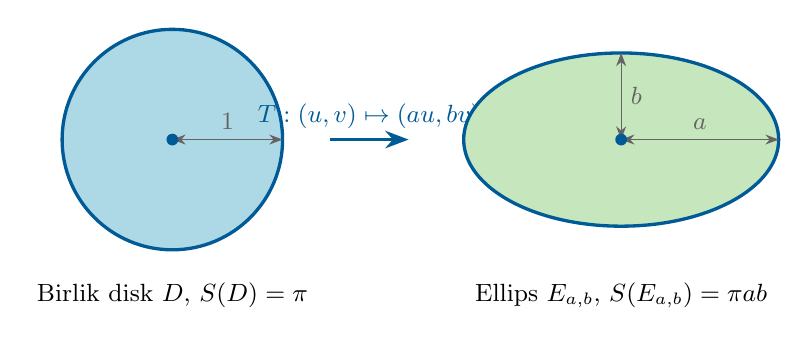
\begin{tikzpicture}
  % Birlik disk
  \begin{scope}[xshift=-3.5cm]
    \fill[fillA] (0,0) circle (1.4);
    \draw[geomblue, very thick] (0,0) circle (1.4);
    \draw[dimline] (0,0) -- (1.4,0) node[midway,above,dimlinelabel] {$1$};
    \node[dotpt] at (0,0) {};
    \node[below, font=\small] at (0,-1.7) {Birlik disk $D$, $\Area{D}=\pi$};
  \end{scope}
  % O'q
  \draw[-Stealth, very thick, geomblue] (-1.5,0) -- (-0.5,0)
    node[midway,above,font=\small] {$T:(u,v)\mapsto(au,bv)$};
  % Ellips
  \begin{scope}[xshift=2.2cm]
    \fill[fillC] (0,0) ellipse (2.0 and 1.1);
    \draw[geomblue, very thick] (0,0) ellipse (2.0 and 1.1);
    \draw[dimline] (0,0) -- (2.0,0) node[midway,above,dimlinelabel] {$a$};
    \draw[dimline] (0,0) -- (0,1.1) node[midway,right,dimlinelabel] {$b$};
    \node[dotpt] at (0,0) {};
    \node[below, font=\small] at (0,-1.7) {Ellips $E_{a,b}$, $\Area{E_{a,b}}=\pi ab$};
  \end{scope}
\end{tikzpicture}
\caption{Affin o'zgarish: birlik diskdan ellipsga; yuza $ab$ marta oshadi}
\label{fig:ellipse}
\end{figure}

% ============================================================
\section{Parabola segmenti: Arximed kvadraturasi}
\label{sec:archimedes}
% ============================================================

Ushbu bo'lim \emph{ijodiy qism} sifatida keltirilgan:
yuqorida ishlab chiqilgan usullar (uchburchak yuzasi, triangulyatsiya, siqish)
yordamida parabola segmentining yuzasi geometrik hisob bilan aniqlanadi.
Bu natija Arximed ($\approx\,287$--$212$ miloddan avval) tomonidan kashf etilgan
\cite{Archimedes_Heath1897}.

\begin{tarif}[Parabola segmenti]
$y = c - \tfrac{x^2}{4c}$ parabola (yoki umumiy holda $y=cx^2$)
ning biror to'g'ri kesma bilan chegaralangan to'liq qismi
\emph{parabola segmenti} deyiladi.
\end{tarif}

\begin{teorema}[Arximed]
\label{thm:archimedes}
$A$ va $B$ — parabola segmentining uchlarini birlashtiruvchi vatar; $C$ ---
vatar $AB$ ga parallel bo'lgan parabola urinmasining teginish nuqtasi (yoy o'rtasi).
$T = \Area{ABC}$ bo'lsin. U holda:
\[
  \Area{\text{segment}} = \frac{4}{3}\,T.
\]
\end{teorema}
\begin{proof}
\textbf{Asosiy g'oya.}
Har bir qolgan kichik segmentga yangi uchburchakni ``yozilgan'' qilib kiritamiz.
Har bir kichik uchburchakning yuzasi asosiy $T$ ning $\tfrac{1}{4}$ qismiga teng:
bu parabolaning to'rtinchi tartib egrilik xossasidan kelib chiqadi (Arximed uning
``ko'proq'' va ``kamroq'' metodlari bilan isbotlagan \cite{Archimedes_Heath1897}).

\textbf{Geometrik ketma-ketlik.}
$1$-bosqich: $T$ yuzali $\triangle ABC$.
$2$-bosqich: ikkita yangi uchburchak, har biri $\tfrac{T}{4}$ yuzali; jami $\tfrac{T}{2}$.
$3$-bosqich: to'rtta uchburchak, har biri $\tfrac{T}{16}$; jami $\tfrac{T}{4}$. \ldots

\textbf{Yig'indi.}
\[
  \Area{\text{segment}}
  = T\Bigl(1 + \tfrac{1}{4} + \tfrac{1}{16} + \cdots\Bigr)
  = T \cdot \frac{1}{1-\tfrac{1}{4}}
  = \frac{4}{3}\,T. \qedhere
\]
\end{proof}

\begin{figure}[h]
\centering
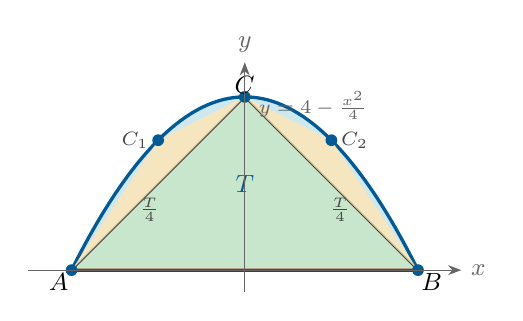
\begin{tikzpicture}[scale=0.55]
  % Parabola y = 4 - x^2/4, -4 <= x <= 4
  % A=(-4,0), B=(4,0), C=(0,4)
  \fill[fillA!60]
    plot[domain=-4:4, samples=80, variable=\x] (\x, {4 - \x*\x/4}) -- cycle;
  \draw[geomblue, very thick]
    plot[domain=-4:4, samples=80, variable=\x] (\x, {4 - \x*\x/4});
  % Vatar AB
  \draw[accred, very thick] (-4,0) -- (4,0);
  % Asosiy uchburchak ABC
  \fill[fillC, opacity=0.7] (-4,0) -- (4,0) -- (0,4) -- cycle;
  \draw[geomgray, thick] (-4,0) -- (4,0) -- (0,4) -- cycle;
  % Kichik uchburchaklar
  \fill[fillD, opacity=0.8] (-4,0) -- (0,4) -- (-2,3) -- cycle;
  \fill[fillD, opacity=0.8] (4,0) -- (0,4) -- (2,3) -- cycle;
  % Nuqtalar
  \node[dotpt] at (-4,0) {};
  \node[dotpt] at (4,0) {};
  \node[dotpt] at (0,4) {};
  \node[dotpt] at (-2,3) {};
  \node[dotpt] at (2,3) {};
  % Etiketlar
  \node[below left, lab] at (-4,0) {$A$};
  \node[below right, lab] at (4,0) {$B$};
  \node[above, lab] at (0,4) {$C$};
  \node[left, font=\scriptsize, geomgray] at (-2,3) {$C_1$};
  \node[right, font=\scriptsize, geomgray] at (2,3) {$C_2$};
  % Yuza etiketlari
  \node[font=\small, geomblue] at (0,2.0) {$T$};
  \node[font=\scriptsize, geomgray] at (-2.2,1.4) {$\tfrac{T}{4}$};
  \node[font=\scriptsize, geomgray] at (2.2,1.4) {$\tfrac{T}{4}$};
  % O'q
  \draw[axisline] (-5,0) -- (5,0) node[right, font=\small] {$x$};
  \draw[axisline] (0,-0.5) -- (0,4.8) node[above, font=\small] {$y$};
  \node[right, font=\scriptsize, dimclr] at (0.1,3.8) {$y=4-\frac{x^2}{4}$};
\end{tikzpicture}
\caption{Arximed kvadraturasi: $\triangle ABC$ ($T$) va birinchi bosqich kichik
         uchburchaklar ($T/4$ har biri)}
\label{fig:archimedes}
\end{figure}

% ============================================================
\section{Xulosa jadvali}
\label{sec:table}
% ============================================================

\begin{table}[h]
\centering
\renewcommand{\arraystretch}{1.5}
\begin{tabular}{@{} l l l @{}}
\toprule
\textbf{Shakl} & \textbf{Yuza formulasi} & \textbf{Asosiy g'oya} \\
\midrule
Kvadrat (tomon $x$)       & $x^2$               & Ta'rif + siqish printsipi \\
To'rtburchak ($a\times b$) & $ab$               & $(a+b)^2$ yoyilmasi \\
To'g'ri burchakli uch. ($a,b$) & $\tfrac{1}{2}ab$ & To'rtburchak yarmi \\
Ixtiyoriy uchburchak ($c, h_c$) & $\tfrac{1}{2}ch_c$ & Balandlik + additivlik \\
Uchburchak (burchak) & $\tfrac{1}{2}ab\sin\gamma$ & Trigonometrik ko'rinish \\
Parallelogramm ($a, h$) & $ah$                & Kesib-ko'chirish \\
Romb ($d_1, d_2$)       & $\tfrac{1}{2}d_1 d_2$ & Diagonallar + 4 uch. \\
Trapetsiya ($a,b,h$)    & $\tfrac{1}{2}(a+b)h$ & Ikkita trap. = parallelogramm \\
Qavariq $n$-burchak    & $\sum_{k=1}^{n-2}\Area{T_k}$ & Triangulyatsiya \\
Doira ($R$)             & $\pi R^2$           & $n$-burchak limiti + ajoyib limit \\
Ellips ($a,b$)          & $\pi ab$            & Affin o'zgarish \\
Parabola segmenti & $\tfrac{4}{3}T$      & Geometrik ketma-ketlik \\
\bottomrule
\end{tabular}
\caption{Tekislik shakllarining yuza formulalari va asosiy g'oyalar}
\label{tab:summary}
\end{table}

% ============================================================
\section{Mashqlar}
\label{sec:exercises}
% ============================================================

Quyidagi masalalar o'rta va yuqori qiyinlikdagi mashqlardan iborat
\cite{Prasolov2006, Apostol1967}.

\begin{enumerate}[leftmargin=*, label=\textbf{\arabic*.}]

\item
$ABCD$ to'g'ri burchakli to'rtburchak bo'lib, $AB=5$ va $BC=3$.
$M$ — $AB$ ning, $N$ — $CD$ ning o'rtasida.
$\Area{AMND}$ ni toping va $\Area{ABCD}$ bilan nisbatini hisoblang.

\item
$ABC$ uchburchakda $AB = 8$, $AC = 6$, $\angle BAC = 60^\circ$.
$\Area{ABC}$ ni hisoblang.
$BC$ ning uzunligini Kosinuslar teoremasidan toping.

\item
Diagonallari $d_1 = 12$ va $d_2 = 5$ bo'lgan rombning perimetri va yuzasini
hisoblang.

\item
Tomoni $a$ bo'lgan muntazam olti burchakning yuzasini triangulyatsiya usulida
hisoblang.
Natijani $\tfrac{3\sqrt{3}}{2}a^2$ bilan solishtiring.

\item
Isbotlang: agar ikkita uchburchak umumiy asosga ega bo'lib, uchinchi uchlarining
mos tushishi mumkin bo'lmasa ham bir xil balandlikka ega bo'lsa, ularning
yuzalari teng.

\item
$a$ tomonli muntazam $n$-burchakka ichki chizilgan doiraning radiusini
$r = \tfrac{a}{2\tan(\pi/n)}$ formula bilan ifodalang va
$\Area{P_n} = \tfrac{1}{2}\,n\cdot a \cdot r$ ekanini ko'rsating.

\item
$x \in \Rplus$ uchun $\Area{Q_x} = x^2$ formulasini quyidagi yo'l bilan qayta
isbotlang: $x_1 < x < x_2$, $x_1, x_2 \in \Qplus$ hol uchun siqish printsipini
to'g'ridan-to'g'ri qo'llang.

\item
Affin o'zgarish $T(u,v)=(2u,\,3v)$ ta'sirida birlik kvadrat ($[0,1]^2$) qanday
shakl hosil qiladi va yuzasi qanchaga ko'payadi?

\item
Arximed kvadraturasida, agar $C$ nuqtasi arc midpoint emas, balki parabola
$y = x^2$ ustidagi ixtiyoriy nuqta bo'lsa, $T = \Area{ABC}$ maksimal qiymati
qaysi $C$ da erishilishini ko'rsating.

\item[\textbf{10*.}]
$ABCDE$ qavariq beshburchak berilgan.
Har bir uchidan diagonal chizib triangulyatsiya qiling va
$\Area{ABCDE}$ ni uchta uchburchak yuzalari yig'indisi sifatida ifodalaydigan
formulani yozing.
Natijani $A_1=(0,0)$, $A_2=(4,0)$, $A_3=(5,3)$, $A_4=(2,5)$, $A_5=(-1,3)$
uchun tekshiring.

\end{enumerate}


\newpage
% ---- Adabiyotlar ----
\printbibliography[heading=bibintoc, title={Adabiyotlar}]

\end{document}
